%!TEX encoding = UTF-8 Unicode
%!TEX TS-program = xelatex

% paper for BeLLS
\documentclass[11pt,twoside]{article}
%!TEX encoding = UTF-8 Unicode
% packages and settings for BeLLS
% all packages are available in standard LaTeX distributions such as MacTeX 2016

% page layout (text area is 126mm, 196mm)
\usepackage[papersize={17cm,24cm},margin=22mm,top=17mm,headsep=5mm]{geometry} 

\usepackage{xltxtra} % extras for XeLaTeX
\usepackage{verbatim} % verbatim input
\usepackage{titling} % customize title
\usepackage{csquotes} % context sensitive quotes
\usepackage{upquote} % allow correct quotes in verbatim
\usepackage[bottom]{footmisc} % put footnotes down at the bottom margin
\usepackage[svgnames]{xcolor} % color pictures with SVG names
\usepackage{graphicx} % \includegraphics
\usepackage{enumitem} % customize lists
%\setitemize{noitemsep,topsep=0pt,parsep=0pt,partopsep=0pt}
\setitemize{itemsep=2pt,topsep=4pt,parsep=0pt,partopsep=0pt}
\usepackage{covington}  % for numbered linguistic examples

%\usepackage[english]{babel} % multilinguality
\usepackage{polyglossia} % newer alternative to babel
\setdefaultlanguage{english} % see http://ctan.uib.no/macros/xetex/latex/polyglossia/polyglossia.pdf

\setmainfont[Mapping=tex-text,Ligatures=TeX,Scale=1.0]{Linux Libertine O} 
\setmonofont[Mapping=tex-text,Scale=MatchLowercase,LetterSpace=-2.0]{DejaVu Sans Mono}
\renewcommand{\baselinestretch}{1.04} % stretch distance between baselines
\frenchspacing % reduce space after sentence-final punctuation
\date{}
\setlength{\parindent}{1em}
\clubpenalty = 10000
\widowpenalty = 10000
\hfuzz = 2pt  % No warnings about margin overhangs less than this amount.
%\setlength{\belowcaptionskip}{-1.2em}

\usepackage[backend=biber, style=authoryear, citestyle=authoryear-comp, maxcitenames=2, maxbibnames=50, language=auto, isbn=false, url=false]{biblatex} % new alternative to bibtex
\setlength{\bibhang}{\parindent}
\usepackage[breaklinks,colorlinks,urlcolor=black,citecolor=black,linkcolor=black]{hyperref} % pagebackref incompatible with biblatex

\usepackage[compact,noindentafter]{titlesec} % customize section headings
\titlespacing{\section}{0pt}{2.7mm}{1.5mm} % left indent, space before, space after
\titlespacing{\subsection}{0pt}{2mm}{1pt}
\titlespacing{\subsubsection}{0pt}{1.2mm}{0.5pt}

\newcommand\Volume{N} % BeLLS Volume number
\newcommand\Voleditors{Jan Editor and Ed Janitor}
\newcommand\Voltitle{The book title}
\newcommand\VolISBN{N}
\newcommand\VolDOI{N}

%\usepackage{natbib}
%\usepackage{fullname}
%\bibliographystyle{fullname} % chicago or spbasic or spmpsci or spphys
%\setlength{\bibhang}{-0.5em}
%\setlength{\bibsep}{0mm}
%\let\bibfont=\small

% footnote without number
\newcommand\blfootnote[1]{
  \begingroup
  \renewcommand\thefootnote{}\footnote{\hspace{-2.4em} #1}%
  \addtocounter{footnote}{-1}
  \endgroup
}

% customize title
\renewcommand{\maketitle}
  {\bgroup\setlength{\parindent}{0pt}
   \begin{flushleft}
    \textbf{\LARGE{\ \\ \vspace{20mm}\strut\thetitle\strut}\vspace{2mm}}
    
    {\Large\theauthor}
  \end{flushleft}\egroup\vspace{18mm}
}

% customize abstract
\renewenvironment{abstract}
  {\noindent\small %\quotation
  {\noindent{\large\textbf\abstractname. }%\par\nobreak\smallskip
  \thispagestyle{plain}
  %\blfootnote{In: \emph{Volume title,} edited by Jan Editor and Ed Janitor. BeLLS Vol. N (2017), DOI N. Open Access under the terms of CC-BY-NC-4.0.}
  }}
  {}
    
% command in which to embed tabular material in numbered example
% use: \begin{example}\extab\begin{tabular ...
\newcommand{\extab}[2][-0.69\baselineskip]{ 
   \parbox[t]{.9\textwidth}{
     \setlength{\tabcolsep}{1.3pt} % use small space between columns
     \vspace{#1}
     #2
    }
}

% command to put ref in parentheses
\newcommand{\refp}[1]{(\ref{#1})}

% customize page headers
\usepackage{fancyhdr}
\pagestyle{fancy}
\renewcommand{\headrulewidth}{0.4pt}
\fancyhead{}  \fancyfoot{} %clear
\makeatletter % necessary for commands with @
  \fancyhead[RO]{\small\textit{\@title}}
  \fancyhead[LE]{\small\textit{\@author}}
\makeatother
%\fancyhead[RE]{\small BeLLS Vol. \Volume}
 % no footer
\setlength{\headheight}{20.68pt} % room for two lines
\fancypagestyle{plain}{% first page of chapter
 %\fancyhead[L]{}
 \fancyhead[L]{\footnotesize In: \emph{Volume title,} edited by Jan Editor and Ed Janitor. BeLLS Vol. N (2017), DOI N. Open Access under the terms of CC-BY-NC-4.0.} % comment to keep the normal header
  \fancyhead[C,R]{}
  %\renewcommand{\headrulewidth}{0pt} % comment to keep rule
  \fancyfoot{} % comment to put page number at bottom
  }

 % load packages, set parameters, define commands


\author{Ian Palacín, Jordi Planes, Simone Arena}
\title{Preliminary report on prediction of failures for the HMC106 centrifugal compressor} % do not capitalize every open class word

\hyphenation{lem-mat-iz-at-ion uni-code ADVdeg Hel-ge}
\graphicspath{{relevant_graphs/}} % the pictures folder

\begin{document}
\maketitle

\section{Introduction}
The aim of this report is to briefly explain a preliminary study of the data provided
by the HMC106 centrifugal compressor and the potential it has when it comes to detecting filures 
before they happen. The benefits of this application are numerous.\\
What is needed to understand the content below will be explained 
throughout the document, so that no previous knowledge is required to understand the general idea.\\
Each section of this document except for the first and the last one will show the results of the
study upon a real different fail of the machine. There will be a total of 4 fails shown:
\begin{itemize}
  \item \textbf{Fail 1} will serve as a point of view of the early stages of the study.
  \item \textbf{Fail 2, 3 and 4} it will serve as a point of view of the late stages of the study. 
\end{itemize}
The first section will explain the most important tools that have been used to generate the results,
which are represented visually by two different graphs. These graphs will appear in each of the fails
that will be seen in this document, so the first section will explain how to interpret them.


\noindent In the appendix there is more information about each fail and the data used to study it.

\newpage
\section{Statistical tools and graphs}
A series of tools and techniques have been used to obtain the data that will be represented in
the graphs, the most important two are the following:
\begin{itemize}
     \item \textbf{PCA:} Principal Component Analysis, brings together different variables into
     one in such a way that it maintains the properties and relations of the original variables.
     Working with one variable instead of many is easier and makes its visual representation
     feasible. \textbf{If you want to know more...} it is a branch of the multivariate statistical
     analysis based on dimensionality reduction. It makes a linear mapping of the data from the 
     eigenvectors of the covariance matrix that correspond to the largest eigenvalues (main 
     components).

     \item \textbf{Mahalanobis distance:} measures the distance of a specific value from the other
     values in the dataset. In other words, it measures how anomalous or "strange" is a specific value
     compared to the rest. \textbf{If you want to know more...} doing the standard deviation we could
     find how anomalous is a value with respect to the center of mass, but we would be assuming that
     the sample points are distributed in a spherical manner. When the distribution is non-spherical,
     for instance ellipsoidal, the probability of the test point depends not only on the center of mass,
     but also on the direction. The Mahalanobis distance consider these details.
\end{itemize}

\noindent In this report, the result of the prediction of a failure is represented by two graphs. These graphs will
be seen in each of the following sections and were obtained using the techniques mentioned above, among
others.
\newpage
\subsection{Anomaly metric}
\begin{figure}[h!]
\centering
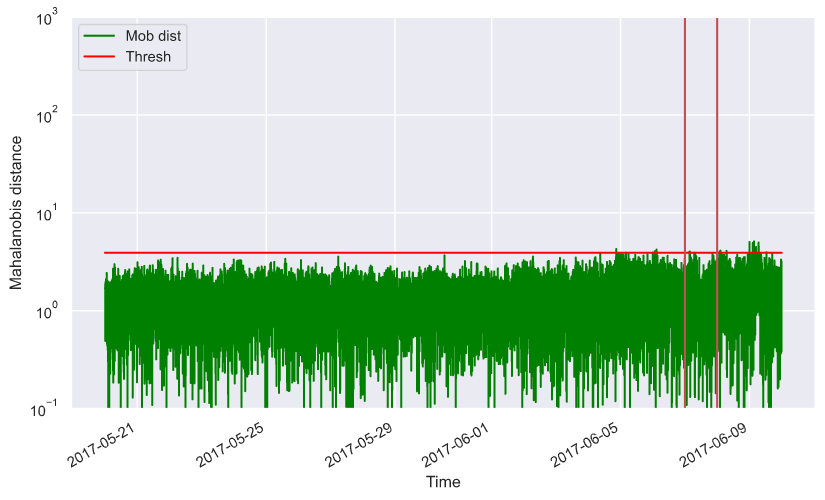
\includegraphics[width=0.65\textwidth]{0_AM_label.png}
\caption{Anomaly metric}\label{screenshots}
\end{figure}
\noindent The first graph is the Anomaly Metric, it is based on the data of a set of variables, for instance,
the temperature and the vibration of the sensor X over a period of time.\\
The \textbf{green line} is the Mahalanobis distance, measuring the "strangeness" of each data point
of the original dataset. The \textbf{two vertical red lines }represent the beginning and the end of the fail
respectively, in this case 24.10.2016 to 27.10.2017. The \textbf{horizontal red line} is an example of a
threshold, where a notification could be sent.\\
It can be interpreted as \textbf{\textit{"how anomalous is each data point over a period of time"}}.

\subsection{Anomaly metric tendency}
\begin{figure}[h!]
\centering
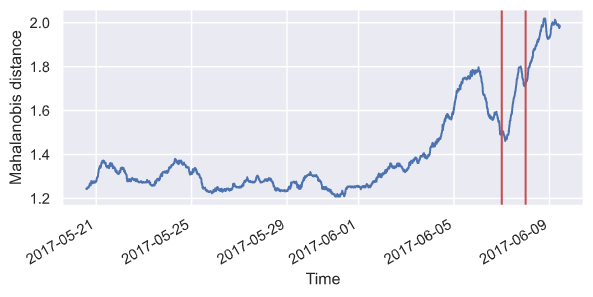
\includegraphics[width=0.8\textwidth]{0_T_label.png}
\caption{Anomaly tendency}\label{screenshots}
\end{figure}
\noindent The second graph is the Anomaly Tendency, it shows the tendency of the Anomaly metric graph.
It is a more visual and intuitive way to see the general path of the previous graph. The beginning and
end of the fail is also represented as the two red vertical lines.\\
It can be interpreted as \textbf{\textit{"how anomalous is the data overall"}}.


\section{Fail 1}
This is the first fail shown in the document, it will serve as a point of view
of the first steps of the study. The machine failed from the 24.10.2016 to the
27.10.2017, the data used to analyze it was the pressure and temperature of the
compressor\footnote{HPI602, HPI605, HTI605}, and revealed the following graphs:\\


\begin{figure}[h!]
\centering
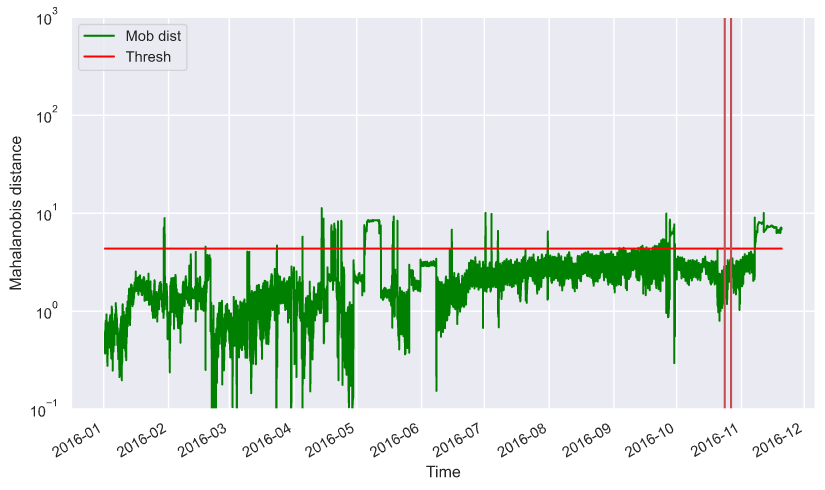
\includegraphics[width=0.65\textwidth]{4_4_AM_label.png}
\caption{Anomaly metric for fail 1}\label{screenshots}
\end{figure}
At the beginning of the study there was a lot of data to filter and to treat,
the variables and the general behavior of the data was not clear and all the 
impediments produced poor results. The poor results can be seen in the graph,
where nothing is clear and no feature can be taken out of it.

\begin{figure}[h!]
\centering
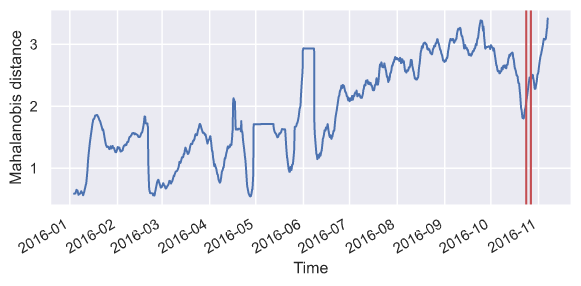
\includegraphics[width=0.65\textwidth]{4_4_T_label.png}
\caption{Anomaly tendency for fail 1}\label{screenshots}
\end{figure}
The same errors are also extrapolated to the second graph, where no failure
is appreciated nor detected.

\newpage
\section{Fail 2}
The fails of the machine that will be shown from now on (3, 3 and 4) will serve as a point of view
of the late stages of this study, where the greater knowledge of the important variables, the
general behavior of the data and the proper treatment of it led to noticeable results.\\
The fail that will be shown in this section started the 22.05.2017 and ended three days later, the
25.05.2017. The data used to analyze the failure is from two variables that represent the axial
displacement of the compressor\footnote{HZI877B, HZI877C}.

\begin{figure}[h!]
\centering
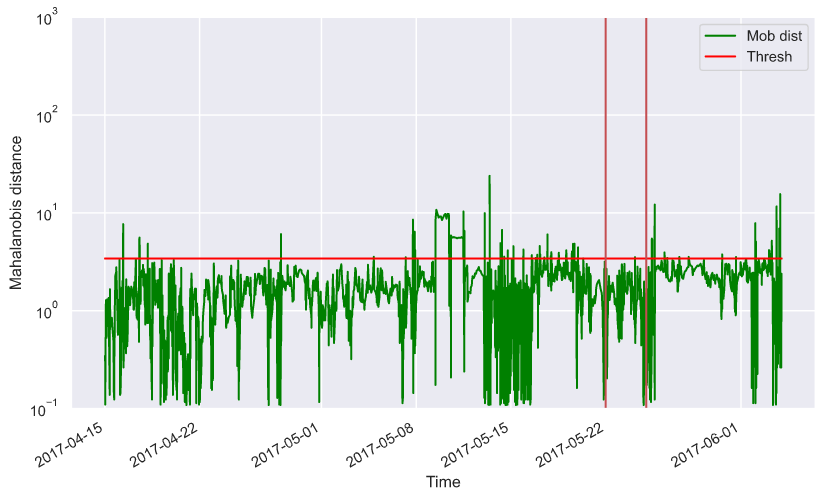
\includegraphics[width=0.65\textwidth]{6_1_AM_label.png}
\caption{Anomaly metric for fail 2}\label{screenshots}
\end{figure}
As the graph below shows how abnormal each data point is separately, the information represented
is difficult to see. That is why we have the second graph, where the general tendency is clear, 
and the results appear more obvious.

\begin{figure}[h!]
\centering
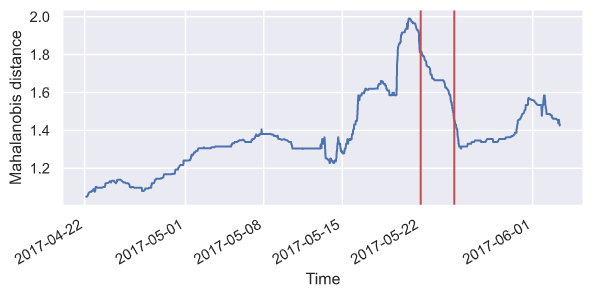
\includegraphics[width=0.65\textwidth]{6_1_T_label.png}
\caption{Anomaly tendency for fail 2}\label{screenshots}
\end{figure}
In the graph above it is clearly seen the exact moment where the machine failed, the peak of 
the curve. An ascendant curve that could be a visual representation of the deterioration of 
the machine (or a part of it), culminating in its failure marked with the first red line. The
fail could have been detected over 10 days in advance.


\section{Fail 3}
The next fail started on the 12.11.2018 and ended on the 29.11.2018. This time the data is based
on the temperature and vibration of the electric motor\footnote{HTI880A, HTI879B, HTI883A, HVI877X, HVI877Y, HVI878Y}.
\begin{figure}[h!]
\centering
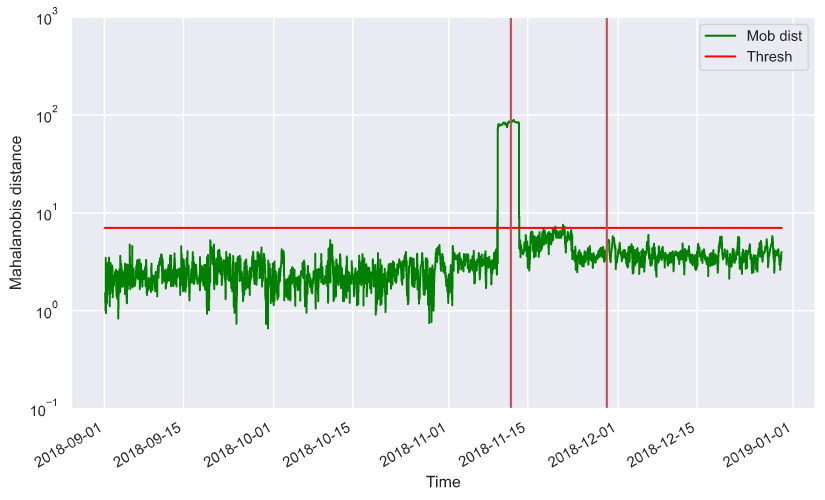
\includegraphics[width=0.65\textwidth]{7_3_AM_label.png}
\caption{Anomaly metric for fail 3}\label{screenshots}
\end{figure}
\begin{figure}[h!]
\centering
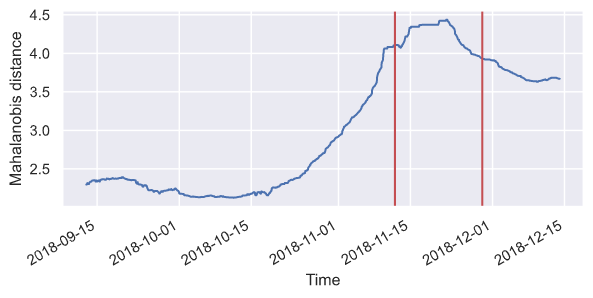
\includegraphics[width=0.65\textwidth]{7_3_T_label.png}
\caption{Anomaly tendency for fail 3}\label{screenshots}
\end{figure}
\newpage
The results are similar to the ones in the previous section, a clear deterioration leading to the 
fail of the machine, foreseeable 10 days before.

\section{Fail 4}
The last failure seen in this document started on the 12.11.2018 and ended on the 29.11.2018. The
data belongs to the electric motor\footnote{HTI879A, HTI879B, HTI883A, HVI877X, HVI877Y, HVI878Y}, also foreseeable.
\begin{figure}[h!]
\centering
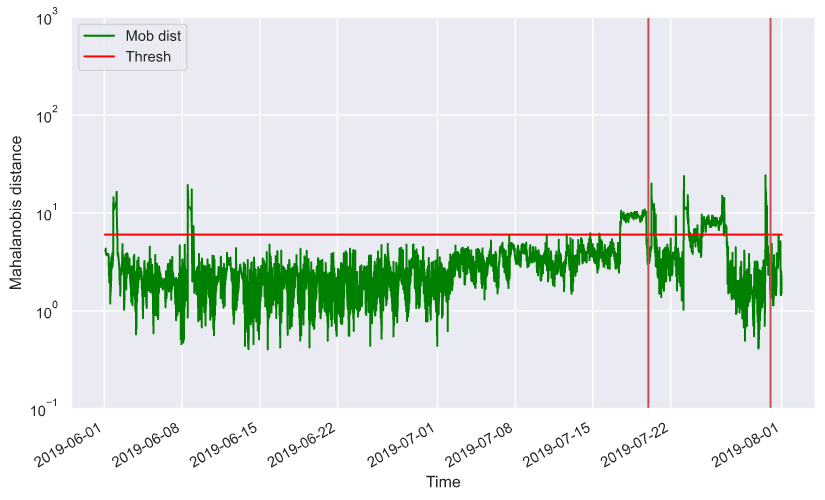
\includegraphics[width=0.65\textwidth]{8_3_AM_label.png}
\caption{Anomaly metric for fail 4}\label{screenshots}
\end{figure}
\begin{figure}[h!]
\centering
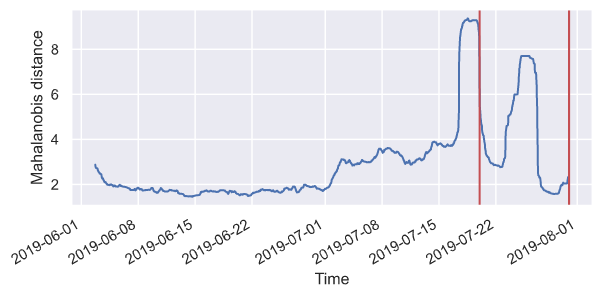
\includegraphics[width=0.65\textwidth]{8_3_T_label.png}
\caption{Anomaly tendency for fail 4}\label{screenshots}
\end{figure}

\newpage
\section{Other insights}
The previous sections showed the capability that the data has at the time
to predict when the machine is going to fail. However, the potential is 
much greater, and the same data can reveal more important information and
insights about the operation of the machine. This information can lead
directly to machine optimizations and better performance. See the following
example.\\
We saw that the data can predict whether the machine is going to fail in a near 
future, but with little effort it can also reduce the number of possible 
culprits of the failure, or even point directly to the specific component that
will cause it. Look at the following graphs:\\
\begin{figure}[h!]
\centering
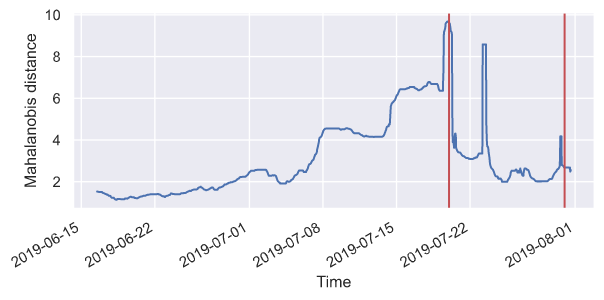
\includegraphics[width=0.65\textwidth]{precedence_1_label.png}
\caption{Anomaly tendency for bearing 892B}\label{screenshots}
\end{figure}
\begin{figure}[h!]
\centering
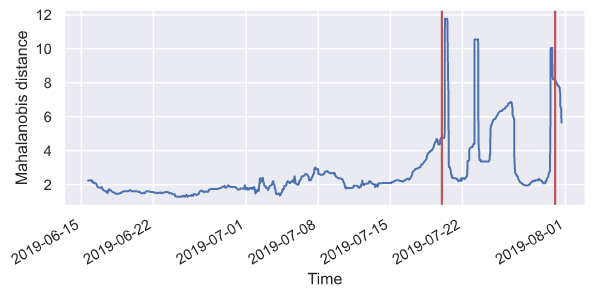
\includegraphics[width=0.65\textwidth]{precedence_2_label.png}
\caption{Anomaly tendency for bearing 891B}\label{screenshots}
\end{figure}
\newpage
Both graphs are from the same machine fail, that of 20.07.2019 to 31.07.2019. They are even from 
the same part of the machine, the gearbox. The difference is that the first is from the 
bearing \textbf{892B}, and the second from the bearing \textbf{891B}. In the first graph 
the deterioration is evident, and the peak occurs \textbf{before} the fail. Contrary 
to the second graph, in which the deterioration is not that obvious, and the peak occurs
\textbf{after} the fail. This type of precedence gives a lot of information about the
culprits of the fail.

\section{Conclusions}
This was only a preliminary study on the data of the machine aimed to show the potential 
and maneuverability that it offers, and the amount of valuable information that could 
provide the continuation of the analysis, with a deeper study of the data.
In this document were just presented a few examples.

\newpage
\section{Appendix A}
\subsection{Details of fail 1} 
\textbf{Variables used}: HPI602, HPI605, HTI605\\
\textbf{Time of the fail}: 24.10.2016 - 27.10.2016\\
\textbf{Training data graphic}:
\begin{figure}[h!]
\centering
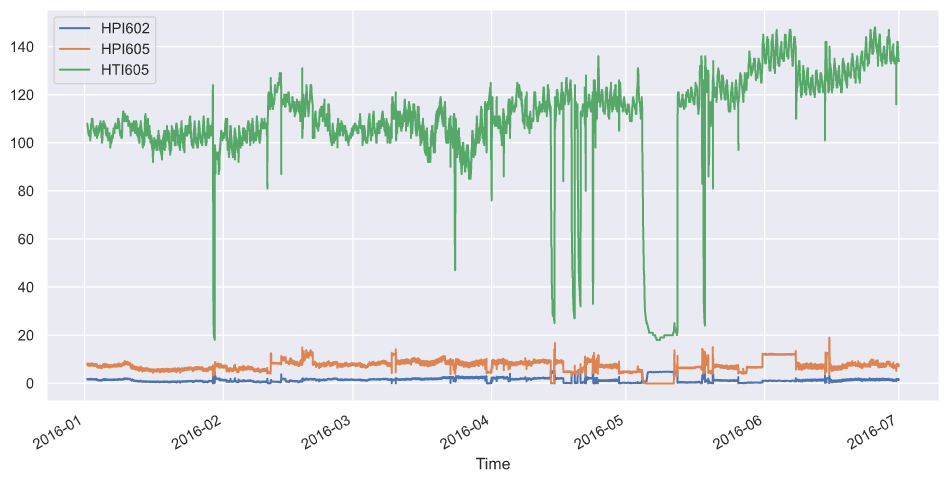
\includegraphics[width=0.65\textwidth]{train_fail0.png}
\caption{Training dataset for fail 1}\label{screenshots}
\end{figure}

\subsection{Details of fail 2}
\textbf{Variables used}: HZI877B, HZI877C\\
\textbf{Time of the fail}: 22.05.2017 - 25.05.2017\\
\textbf{Training data graphic}:  
\begin{figure}[h!]
\centering
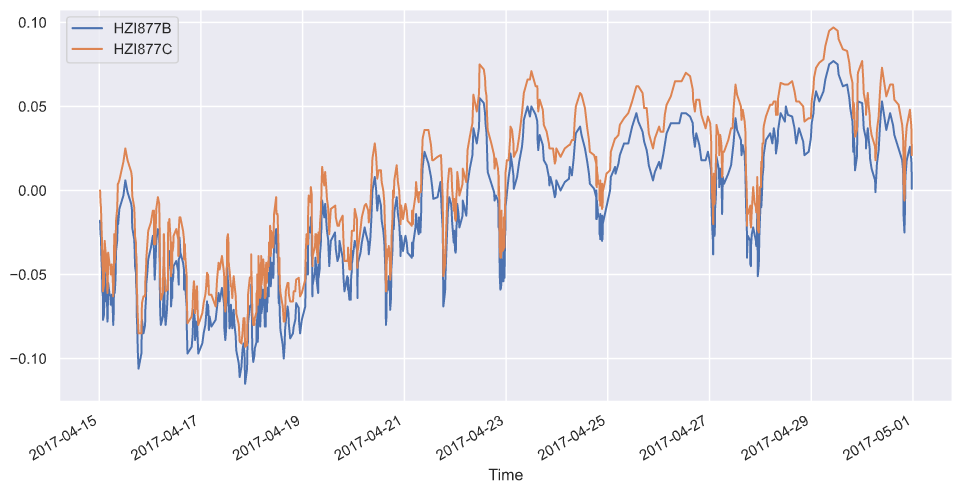
\includegraphics[width=0.65\textwidth]{train_fail1.png}
\caption{Training dataset for fail 2}\label{screenshots}
\end{figure}

\subsection{Details of fail 3}
\textbf{Variables used}: HTI880A, HTI879B, HTI883A, HVI877X, HVI877Y, HVI878Y\\
\textbf{Time of the fail}: 12.11.2018 - 29.11.2018\\
\textbf{Training data graphic}:  
\begin{figure}[h!]
\centering
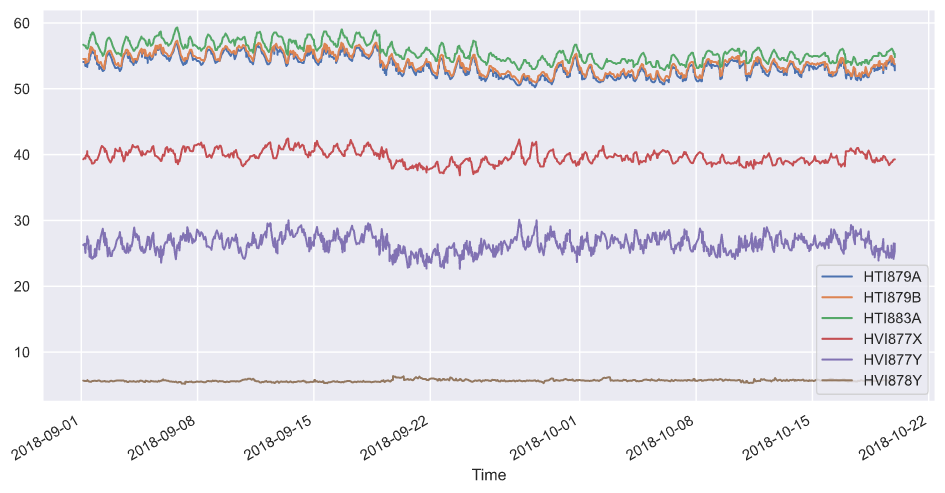
\includegraphics[width=0.65\textwidth]{train_fail2.png}
\caption{Training dataset for fail 3}\label{screenshots}
\end{figure}

\subsection{Details of fail 4}
\textbf{Variables used}: HTI879A, HTI879B, HTI883A, HVI877X, HVI877Y, HVI878Y\\
\textbf{Time of the fail}: 20.07.2019 - 31.07.2019\\
\textbf{Training data graphic}:  
\begin{figure}[h!]
\centering
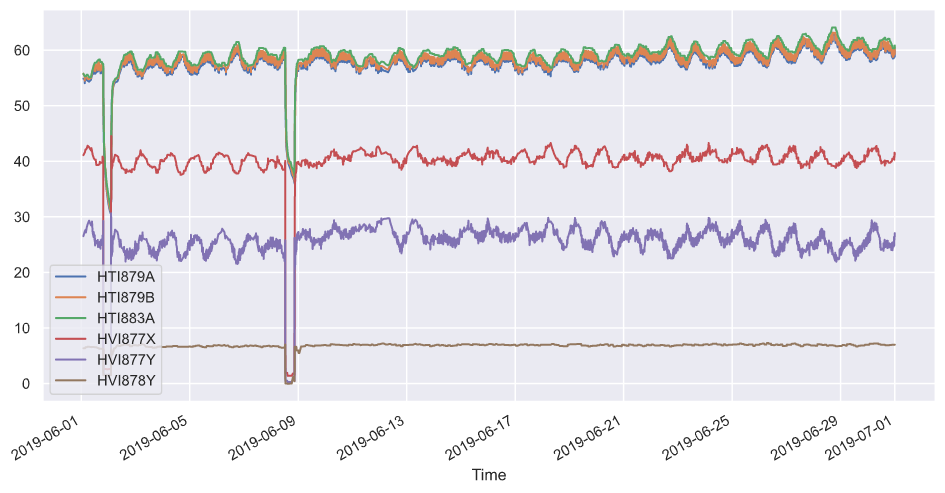
\includegraphics[width=0.65\textwidth]{train_fail3.png}
\caption{Training dataset for fail 4}\label{screenshots}
\end{figure}

\end{document}
